\documentclass{article}
\usepackage[ngerman]{babel}
\usepackage{ucs}
\usepackage[utf8x]{inputenc}
\usepackage{csquotes}
\usepackage{graphicx}
\PassOptionsToPackage{hyphens}{url}\usepackage{hyperref}
\usepackage{lmodern}
\usepackage[T1]{fontenc}
\usepackage{float}

\title{Autonomes RC-Auto mit Kamera}
\author{Anton Bracke}

\begin{document}
\graphicspath{ {./images/} }
\maketitle
\newpage
\tableofcontents
\newpage

\section{Idee und Ziel des Projektes}

Zu Beginn des Wahlmodules \textit{IOT AG} an der Fachhochschule Kiel sollten sich die Studierenden für ein Projekt,
welches über das Wintersemester 2020 / 21 durchzuführen war, entscheiden. Dabei sollten die Schwerpunkten
\textit{Internet of Thing} (kurz IOT), \textit{Microcontroller} und \textit{Sytem-On-a-Chip} (kurz SoC) behandelt werden.
\\~\\
Einer der Teilnehmer entschied sich dabei für ein Projekt bei dem ein ferngesteuertes Auto (folgend RC-Auto) verschiedene Ziele
ansteuern kann. Dabei soll das Auto anlog zu den Systemen von handelsüblichen Staubsaugrobotern zurück zu einer Basisstation
navigieren können.

\section{Projektplanung und Konzeption}

\subsection{Möglichkeiten der Navigation im Innenraum}

Es gibt verschiedenste Ansätze und Verfahren, um auf ein erkanntes oder vordefiniertes Ziel zuzusteuern.
Die Navigation lässt sich dabei entweder durch eine relative Steuerung oder durch den Vergleich von absoluten Positionen umsetzen.
Relativ wäre dabei zum Beispiel: Der Tisch, auf den das Fahrzeug zusteuern möchte, liegt 10 Meter auf 240° von der aktuellen
Position entfernt.
Bei einer Navigation auf Basis von absoluten Positionen kann man zum Beispiel die Luftlinie zwischen zwei GPS-Punkten als Route benutzen.
Dabei wäre dann zum Beispiel die erste Position die des Fahrzeuges und die zweite die des Tisches.

\subsection{Navigation mit Hilfe von Bilderkennung}

Ein typisches System zur Navigation, welches oft von Staubsaugrobotern verwendet wird, basiert auf einer Infrarot-LED
an der Ladestation, welche von einem auf dem Roboter befindlichen 360° IR-Empfänger entdeckt werden kann.
Da für den Betrieb eines solchen Systemes üblicherweise eine Spannungsversorgung für den Roboter und für die Basisstation
notwendig ist, entschied sich der Teilnehmer für eine alternative Variante der Navigation. Bei dieser kommen die Ziele
wie zum Beispiel eine Basisstation ohne Spannungsversorgung oder sonstige aufwendige Installationen aus.
\\~\\
Bei der gewählten Variante wird das RC-Auto mit einer Kamera ausgestattet, welche über einen Livestream Bilder
an einen externen Computer schickt. Dieser erkennt dann auf den Bildern Marker, welche in diesem Fall als Navigationsziele
genutzt werden und sendet Steuerbefehle zurück an das Auto. Hierdurch steurt das Auto solange auf die erkannten Ziele zu,
bis es kurz vor diesen hält. Als Livestream-Kamera lässt sich bereits ein vergleichsweise sehr günstiger Microcontroller mit dem Namen
\textit{ESP32-Cam \footnote{\url{https://randomnerdtutorials.com/esp32-cam-video-streaming-face-recognition-arduino-ide/}}} verwenden,
welcher neben einem Kameramodul zusätzlich über eine W-Lan Verbindung verfügt. Ein Vorteil ist dabei, dass der ESP mit einer
realtiv kleinen Stromversorgung in Form eine Akkus, welcher auf dem eigentlichem Auto mitfahren kann, auskommt.
Die Marker, welche angesteuert werden sollen, können als einfache Bilder auf Papier gedruckt werden und benötigen verglichen
zu einem IR System  somit keine Spannungsversorgung. Zusätzlich ist \enquote{nur} ein externer Computer für die Bilderkennung notwendig.
Mit einem \textit{Raspberry PI \footnote{\url{https://www.raspberrypi.org/products/raspberry-pi-4-model-b/}}} lässt sich aber auch hier
ein vergleichsweise sehr kostengünstiger Aufbau realisieren.

\section{Umsetzung}

\subsection{Bau des RC-Autos}

\begin{figure}[H]
  \begin{center}
    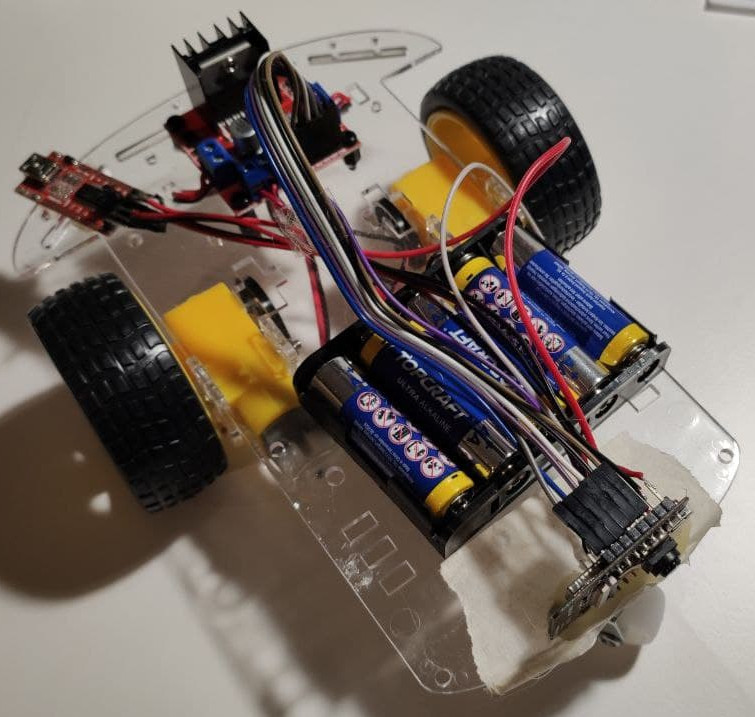
\includegraphics[width=0.75\textwidth]{auto}
    \caption{RC-Auto}
  \end{center}
\end{figure}

Das gesamte Projekt lässt sich für ca 40€ zuzüglich der Kosten für einen externen Computer (minimum Raspberry PI für \textasciitilde50€) nachbauen.
Dabei wird auf einem RC-Auto Bausatz für \textasciitilde15€ die weitere Elektronik verbaut. Der Bausatz besteht aus einer Basisplatte,
zwei Motoren mit Rädern und einem rotierendem Frontrad. Als \enquote{Herzstück} des Autos wird der Microcontroller
\textit{ESP32-Cam} für \textasciitilde12€ eingesetzt. Dieser verfügt über eine kleine Kamera
und ein W-Lan Modul. Flashen lässt sich dieser Microcontroller mit Hilfe eines \textit{FTDI}-Adapters,
welcher \textasciitilde5€ kostet. Für die Motorsterung wird eine H-Brücke vom Typ \textit{L289n} für \textasciitilde10€ genutzt.

\subsection{Motorsterung per Puls-Weiten-Modulation}

Die Motoren des Autos werden mit Hilfe eines speziellen Bauteils, einer so genannten H-Brücke angetrieben.

\begin{figure}[H]
  \begin{center}
    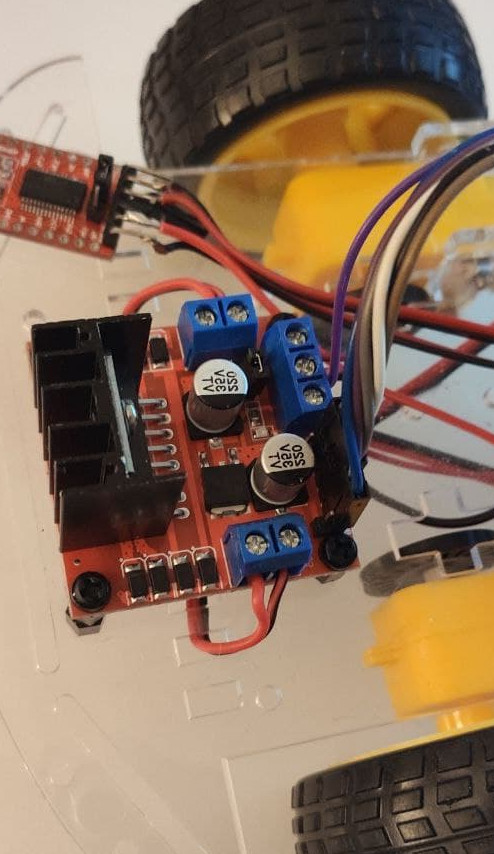
\includegraphics[width=0.5\textwidth]{l298n}
    \caption{H-Brücke (L289n)}
  \end{center}
\end{figure}

Die hier verwendete H-Brücke \textit{L289n} kann zwei Motoren individuell steuern. Über jeweils zwei Digitalpins kann man die Richtung
eines Motors festlegen. \textit{Aus - Aus} oder \textit{An - An} bremst den Motor und bei \textit{Aus - An} und \textit{An - Aus}
dreht der Motor vor- oder rückwärts. Die Geschwindigkeit der Motoren lässt sich zusätzlich über einen
Puls-Weiten-Modulations (kurz PWM) Eingang steuern.

PWM ist eine Modulation bei der über das Verhältnis zwischen An- und Auszeit eines Signales die Weite eines Pulses festgelegt wird. Wenn nun
zum Beispiel im Verhältnis 10\% der Zeit das Signal auf an hat und 90\% der Zeit das Signal aus ist,
so kann man das Signal mit einen vergleichbaren Wert von 10\% interpretieren.

\begin{figure}[H]
  \begin{center}
    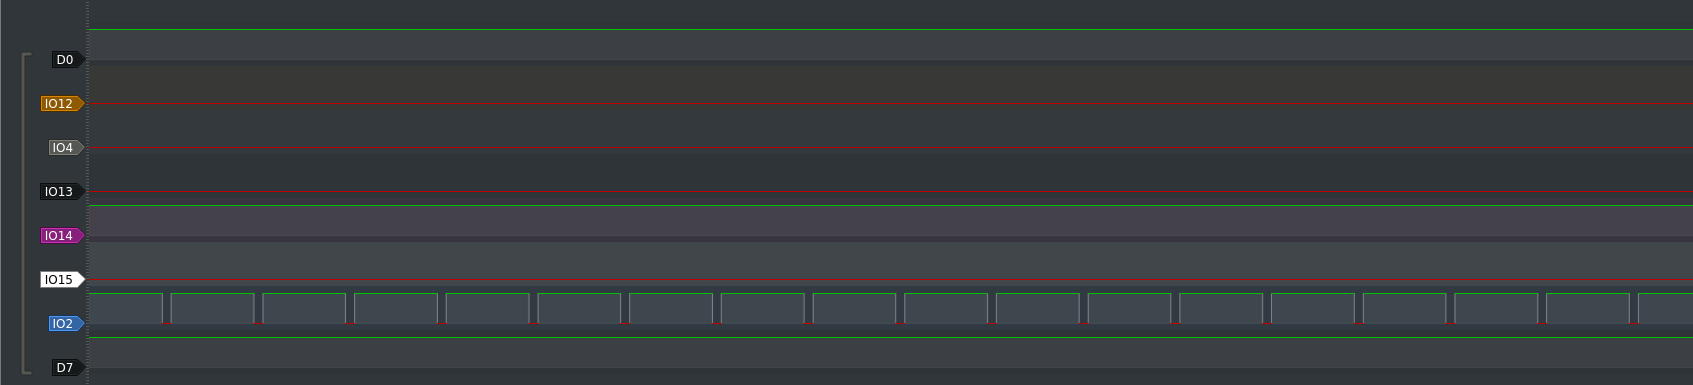
\includegraphics[width=0.75\textwidth]{pwm}
    \caption{PWM-Signal von 98\% aufgenommen mit Logik-Analyser}
  \end{center}
\end{figure}

Zum Steuern des RC-Autos wird auf dem ESP32 einen TCP-Socket\footnote{\url{https://de.wikipedia.org/wiki/Transmission_Control_Protocol}}
auf dem Port \textit{1337} geöffnet. Dieser TCP-Server kann dafür verschiedene Befehle entgegennehmen. Ein Befehl besteht aus mehreren Zeichen,
die mit einer neuen Zeile \enquote{\textbackslash n} beendet werden. Das erste Zeichem stellt dabei die Befehlsart dar.
Ein Befehl zur Steuerung eines Motors ist dabei wie folgt aufgebaut.
Er ist vier Zeichen lang und beginnt mit \enquote{L} oder \enquote{R} für die Auswahl des linken oder rechten Motors,
gefolgt von einem \enquote{+} für Vorwärts oder einem \enquote{-} für Rückwärts. Die letzten 2 Zeichen sind eine Wert in Prozent, der die
Drehzahl des gewählten Motors angibt. Der Befehl \enquote{L-42} würde zum Beispiel den linken Motor mit 42\% rückwärts drehen lassen.
Zum Stoppen des linken Motors kann sowohl der Befehl \enquote{L-00} wie auch \enquote{L+00} genutzt werden. Um beide Motoren direkt zu
stoppen reicht ein einfaches \enquote{!} als Befehl, welcher besonders in der Testphase genutzt wurde.

\subsection{Aruco Marker}

Für die anzusteuernden Ziele des Projektes wurden die sogenannten \textit{Aruco}-Marker verwendet.
Diese sind ählich, wie von QR-Codes bekannt, schwarz-weiß Marker, welche meist in einer Größe von 4x4cm verwendet werden.

\begin{figure}[H]
  \begin{center}
    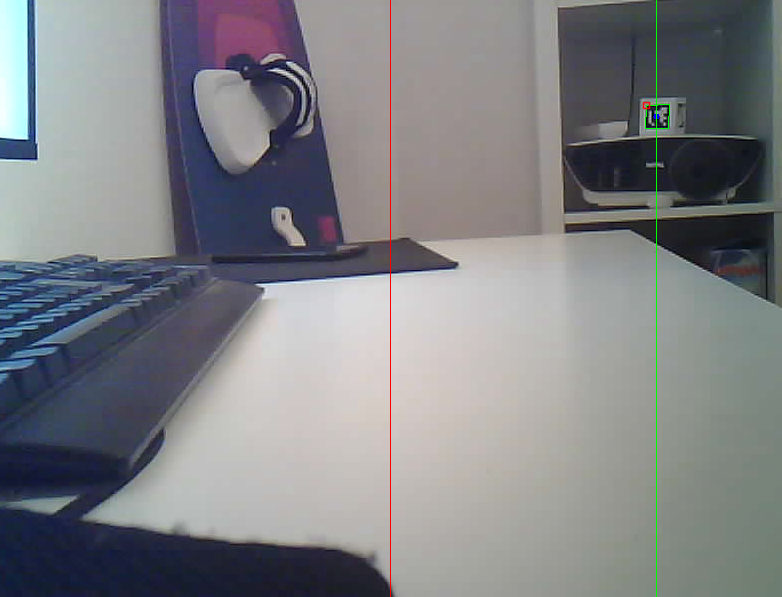
\includegraphics[width=0.75\textwidth]{detect.png}
    \caption{Aruco-Marker in weiter Entfernung}
  \end{center}
\end{figure}

Durch ihr einfaches binäres Muster lassen sich die Marker schnell durch einfache Filter entdecken und ermöglichen es anschließend,
dass durch ihre Verzerrung und Position im 2D Bild die ausgehende 3D Pose geschätzt werden kann. Eine Pose beinhaltet dabei zusätzlich
zur Position noch die Ausrichtung zu einem Ursprung. In diesem Fall wird der Kamerahauptpunkt als Ursprung verwendet.
Um die Pose des Markers im Verhältnis zur Kamera zu schätzen, verwendet man zusätzliche Daten,
die über das Bild bekannt sind. Diese beinhalten die Kalibierungen des Hauptpunktes,
die Brennweite und die Verzerrung der Kamera mit denen das Bild aufgenommen wurde.

\begin{figure}[H]
  \begin{center}
    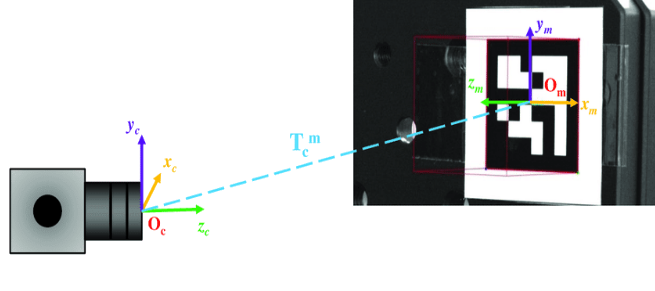
\includegraphics[width=0.75\textwidth]{aruco-detection}
    \caption{Pose zu Aruco-Marker schätzen
    Quelle: \url{https://www.researchgate.net/figure/The-estimation-of-the-position-and-orientation-of-an-ARUCO-18-19-fiducial-marker-and_fig1_327482445} [aufgerufen 26 Feb, 2021]}
  \end{center}
\end{figure}

\subsection{Posenbestimmung und Steuerungs-Regler}

Nachdem nun die Pose eines Markers bestimmt wurde, berechnet ein Computer welche Sterungsbefehle an das RC-Auto gesendet werden müssen,
damit dieses auf den Marker / das Ziel zufährt.

\begin{figure}[H]
  \begin{center}
    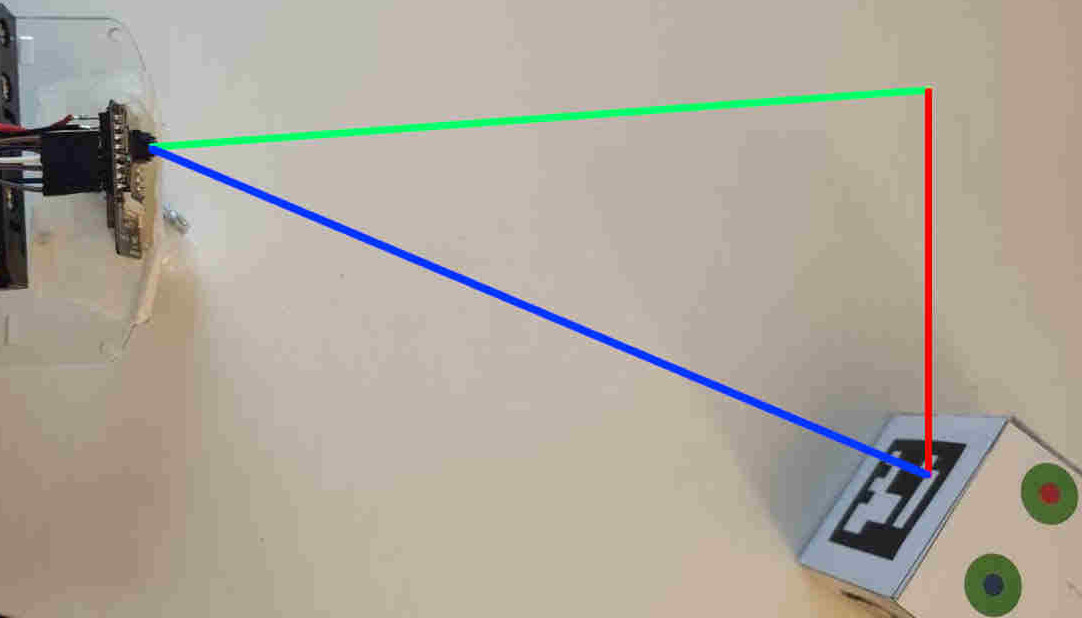
\includegraphics[width=0.75\textwidth]{auto-aruco}
    \caption{Position RC-Auto und Ziel (Aruco-Marker)}
    \label{fig:auto-aruco}
  \end{center}
\end{figure}

Die Steuerung des Autos basiert auf zwei Werten des erkannten Markers, wie in \autoref{fig:auto-aruco} zu sehen.

Dabei wird die Entfernung
zu dem Marker (hier grün) als Basiswert für die Geschwindigkeit verwendet. Die Entfernung, welche in Metern vorliegt, wird in einen Prozentwert
umgerechnet. Unter \textit{20cm} Entfernung wird ein Wert von \textit{0\%} angenommen, sodass das Auto stehen bleibt.
Die restlichen Werte werden von Metern auf Werte von \textit{1\%} bis \textit{99\%} umgerechnet,
wobei zwei Meter die maximale Geschwindigkeit (99\%) darstellen.

Der zweite Wert mit dem das Auto gesteuert wird, ist die Abweichung des Markers zur Fahrtrichtung des Autos (hier rot).
Diese wird zu einem $\pm$ Prozentwert konvertiert und anschließend auf die Basisgeschwindigkeit des Motors addiert.
Dabei wird ein maximalen Lenkwert von \enquote{$\pm 5\%$} genutzt.

\begin{figure}[H]
  \begin{center}
    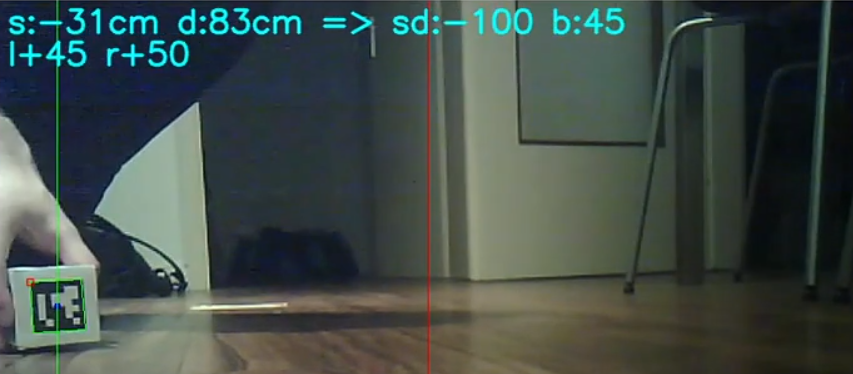
\includegraphics[width=0.75\textwidth]{control}
    \caption{Beispiel Steuerungsberechnung}
    \label{fig:control}
  \end{center}
\end{figure}

Ein Beispiel wie diese Motorensteuerung aus diesen Werten berechnet wird ist in der vorheringen \autoref{fig:control} dargestellt.
Der mit \enquote{s} bezeichnete Wert stellt die Abweichung zur Mitte in \textit{cm} dar. Der Wert mit dem Namen \enquote{d} gibt die
Entfernung vom Marker zum Auto in \textit{cm} an und \enquote{sd} gibt den Lenkfaktor in \% und \enquote{bs} die Basisgeschwindigkeit an.
In der zweiten Zeile sieht man die daraus resultierenden Befehle, welche an das Auto geschickt werden.

\section{Fazit}

Zusammenfassend war das Projekt ein Erfolg und zeigt, wie man mit einer kostengünstigen und einfach aufgebauten Kamera ein autonomes Fahrzeug
bauen kann, welches Aruco-Markern folgt bis es direkt vor diesen zum Stehen kommt.
Um ein derartikes System produktiv einzusetzen wäre es notwenig, die Anwedung zum Beispiel durch ein Algorithmus robuster gegen
mögliche \enquote{Fehler} in der Bildverarbeitung zu machen.

\end{document}